\documentclass[11pt,a4paper]{article}

\usepackage[margin=1in]{geometry}
\usepackage{titlesec}
\usepackage{enumitem}
\usepackage{hyperref}
\usepackage{parskip}
\usepackage{graphicx}
\usepackage{float}
\usepackage{booktabs}
\usepackage{amsmath}

\hypersetup{colorlinks=true, linkcolor=blue, urlcolor=blue}

\titleformat{\section}{\large\bfseries}{\thesection}{0.5em}{}
\titleformat{\subsection}{\normalsize\bfseries}{\thesubsection}{0.5em}{}
\setlist{leftmargin=1.4em, topsep=2pt, itemsep=2pt}

\title{\vspace{-1.5cm}\textbf{PKCERT AI \& Software Development Internship \\ Task 21: Regularization Techniques in Deep Learning}}
\author{Abdullah Amir}
\date{AI and Software Development \\ 31 July 2026}

\begin{document}

\maketitle
\vspace{-0.8cm}

This report covers the theory and the results. The full code and outputs live in the
notebook \texttt{regularization.ipynb}. \textbf{PyTorch 2.13.0 (CPU build), torchvision
0.28.0} are used throughout, random seed \textbf{42} fixed for the split, every model's
initialisation, and training. This task continues directly from Task 20's Fashion-MNIST
feedforward pipeline: Task 20's right-sized network barely overfit, which is the wrong
setting to demonstrate what Dropout, Batch Normalization and Early Stopping actually
fix. This report's baseline is deliberately wider and trained longer, so the
overfitting each technique addresses is real, measured, and visible in the results
below -- not asserted.

% ----------------------------------------------------------------
\section*{Part A: Dataset Selection \& Preparation}

\textbf{Dataset}: Fashion-MNIST (Xiao, Rasul \& Vollgraf, 2017), the same 70,000
$28\times28$ greyscale clothing images across 10 classes used in Task 20. Reusing it is
deliberate: it lets this task's deliberately-overfitting baseline be judged against
Task 20's already-established right-sized network on identical data.

\textbf{Three-way split}: the official 10,000-image test set is held out completely
until final evaluation. The official 60,000-image training set is split
\textbf{50,000 (71.4\%) train / 10,000 (14.3\%) validation}, seed 42. Normalization
statistics (mean = 0.2857, std = 0.3529) are computed from the training split only, as
established in Task 20. Each image is flattened to a 784-dimensional vector, batched at
size 256.

% ----------------------------------------------------------------
\section*{Part B: Model Development}

\textbf{Baseline architecture: $784 \to 512 \to 256 \to 10$} (2 hidden layers, ReLU, no
regularization at all) -- roughly \textbf{4x} the parameter count of Task 20's
right-sized network, trained on the identical 50,000 images. That capacity-vs-data
imbalance is what produces clear overfitting. Optimizer: Adam(lr=$10^{-3}$). Loss:
CrossEntropyLoss. Batch size 256, 25 epochs, no early stopping in this baseline run, so
the full overfitting trajectory is visible.

\begin{figure}[H]
    \centering
    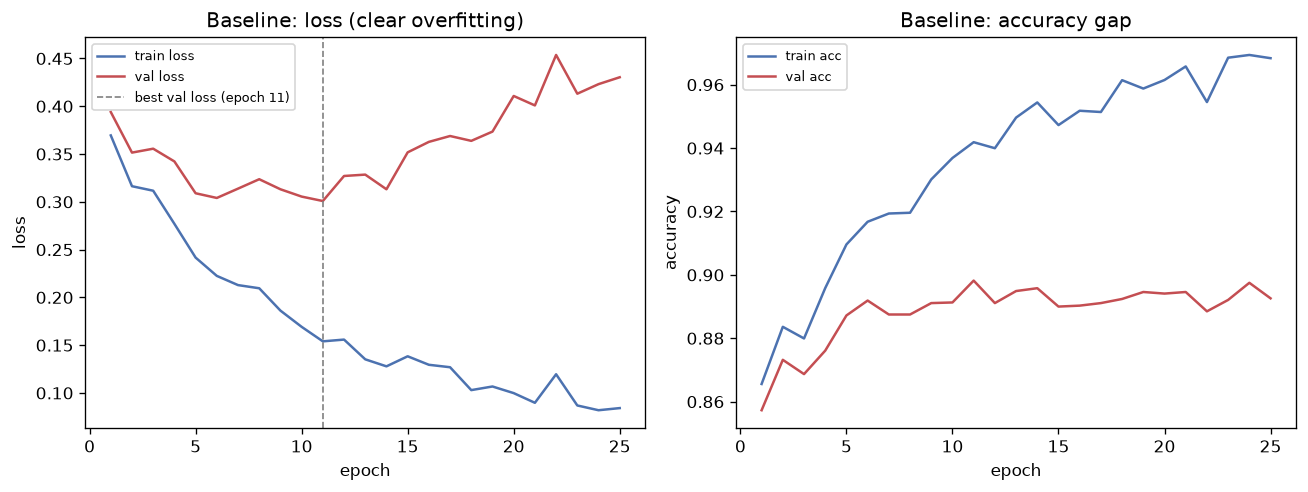
\includegraphics[width=0.95\textwidth]{figures/01_baseline_overfitting.png}
    \caption{Baseline loss and accuracy curves. Validation loss is lowest at epoch 11
    (0.3008) and rises to 0.4304 by epoch 25; the train/validation accuracy gap widens
    steadily throughout training.}
\end{figure}

\textbf{Confirmed, not assumed}: validation loss bottoms out at epoch 11 and then rises
for the remaining 14 epochs; the final train/validation accuracy gap is
\textbf{+0.0758} (train 0.9684 vs val 0.8926, both at the final epoch) -- a
substantially larger and clearer overfitting signature than Task 20's right-sized
network showed, exactly as intended.

\begin{table}[H]
\centering
\begin{tabular}{lr}
\toprule
\textbf{Metric (test set, baseline)} & \textbf{Value} \\
\midrule
Accuracy & 0.8874 \\
Macro-F1 & 0.8876 \\
\bottomrule
\end{tabular}
\end{table}

% ----------------------------------------------------------------
\section*{Part C: Regularization Techniques}

All three techniques, plus a combined configuration, share the baseline's architecture
skeleton, optimizer, batch size, seed and epoch budget (25, unless early stopping
triggers first), so the comparison isolates the regularization technique itself.

\textbf{C1: Dropout} (p=0.5 after each hidden layer's activation).
\textbf{C2: Batch Normalization} (\texttt{BatchNorm1d} after each linear layer, before
ReLU). \textbf{C3: Early Stopping} (patience=5 on validation loss, applied to the plain
baseline architecture, restoring the best-validation-loss weights).

\begin{figure}[H]
    \centering
    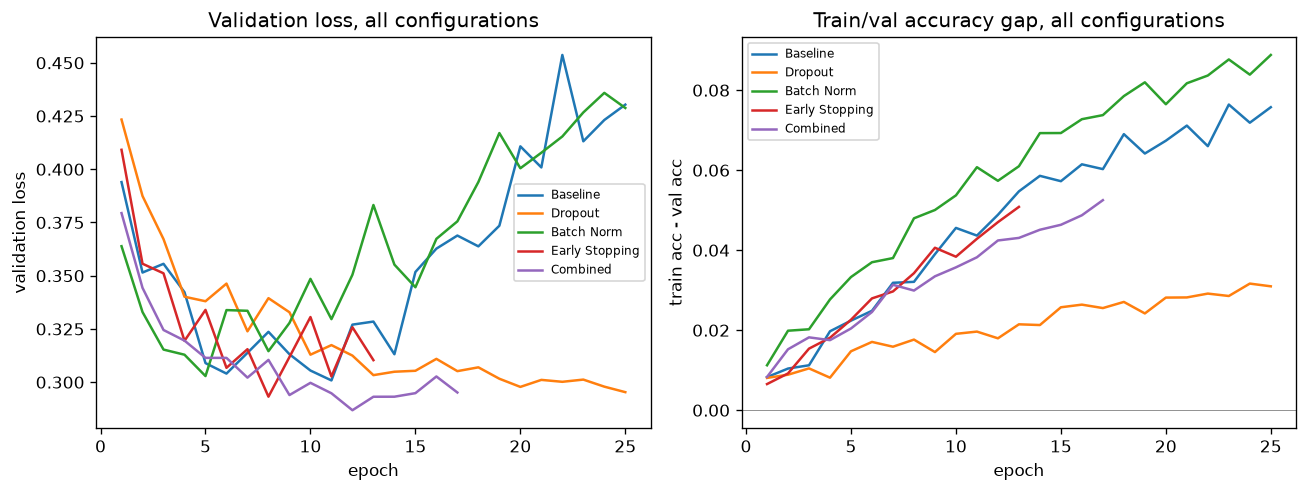
\includegraphics[width=0.95\textwidth]{figures/02_all_loss_curves.png}
    \caption{Left: validation loss for all five configurations. Right: train/validation
    accuracy gap for all five. Dropout's gap stays flattest throughout; Batch Norm's
    grows fastest of all.}
\end{figure}

\begin{table}[H]
\centering
\begin{tabular}{lrrrrr}
\toprule
\textbf{Configuration} & \textbf{Test Acc} & \textbf{Test F1} & \textbf{Train/Val Gap} & \textbf{Epochs} & \textbf{Time} \\
\midrule
Baseline & 0.8874 & 0.8876 & 0.0758 & 25 & 352.3s \\
Dropout (p=0.5) & 0.8879 & 0.8868 & \textbf{0.0310} & 25 & 344.0s \\
Batch Normalization & \textbf{0.8914} & \textbf{0.8916} & 0.0888 (worst) & 25 & 360.4s \\
Early Stopping & 0.8896 & 0.8895 & 0.0508 & 13 & \textbf{176.7s} \\
Combined (Dropout+BN+ES) & 0.8901 & 0.8907 & 0.0525 & 17 & 241.7s \\
\bottomrule
\end{tabular}
\caption{All five configurations, identical seed/optimizer/architecture skeleton, tested on the same held-out 10,000-image test set.}
\end{table}

\begin{figure}[H]
    \centering
    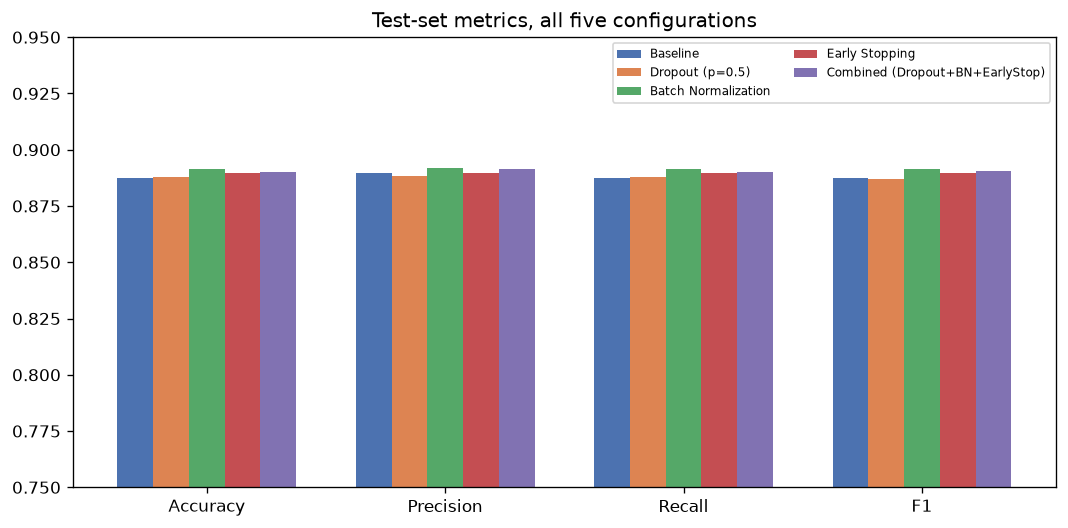
\includegraphics[width=0.78\textwidth]{figures/03_metrics_comparison.png}
    \caption{Accuracy, precision, recall and F1 across all five configurations -- all cluster within about 0.4 points of each other.}
\end{figure}

\begin{figure}[H]
    \centering
    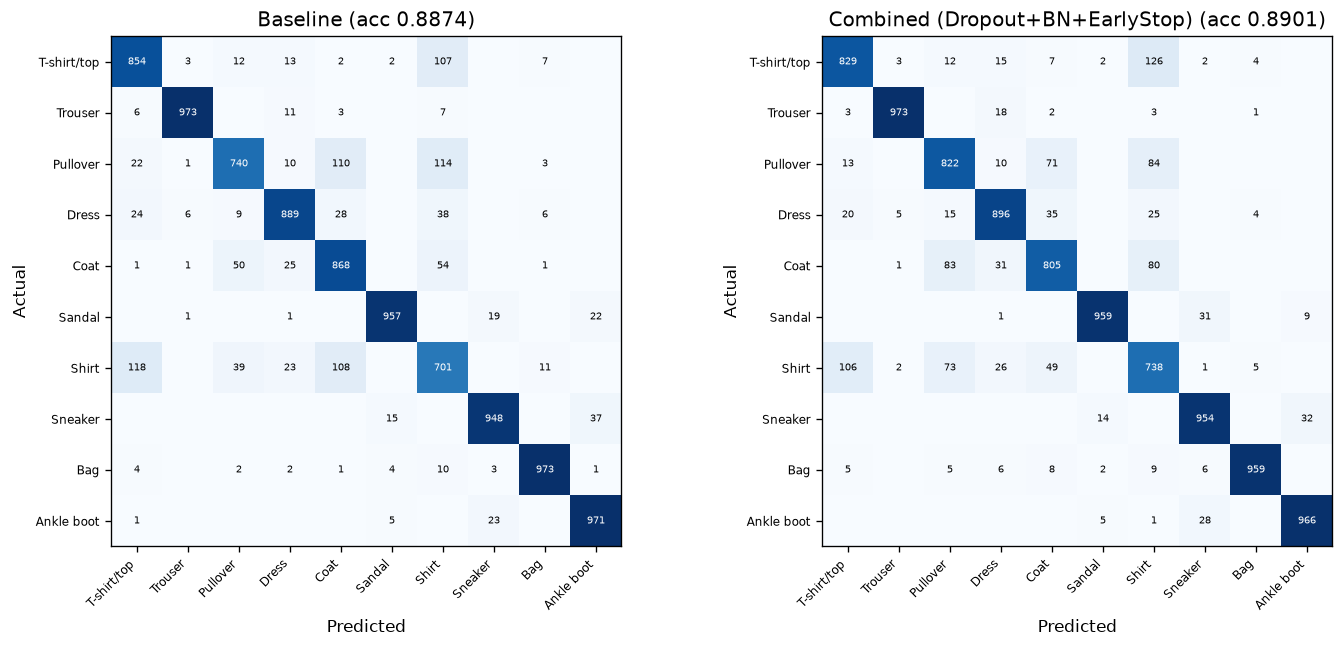
\includegraphics[width=0.95\textwidth]{figures/04_confusion_matrices.png}
    \caption{Confusion matrices, baseline vs the combined configuration. Both show the
    same Shirt/T-shirt/top/Pullover/Coat confusion cluster identified in Task 20; the
    combined model's error pattern is similar in shape, not fundamentally different --
    regularization changed the degree of overfitting, not which classes are hard.}
\end{figure}

\textbf{Three results here, and none of them is the naive story.}

\textbf{Dropout cut the overfitting gap roughly in half} (0.0758 $\to$ 0.0310) but
barely moved test accuracy (0.8874 $\to$ 0.8879) -- it did exactly what dropout is
supposed to do, regularize, with only a marginal accuracy payoff on this particular
dataset and model size.

\textbf{Batch Normalization gave the best raw test accuracy of any single technique
(0.8914) but its overfitting gap was the \emph{worst} of all five} (0.0888, worse than
even the unregularized baseline's 0.0758). This is the genuinely counter-intuitive
result of this task, returned to in Part D: Batch Normalization's popular reputation as
a regularizer was not borne out here. It clearly helped optimization -- faster, more
stable convergence to a better optimum, which is what raised its accuracy -- but it did
not reduce the variance between training and validation performance the way Dropout and
Early Stopping did.

\textbf{Early Stopping improved on the baseline on every axis simultaneously}: better
test accuracy (0.8874 $\to$ 0.8896), a much smaller gap (0.0758 $\to$ 0.0508), and
\textbf{half the training time} (352.3s $\to$ 176.7s), for zero added architectural
complexity -- it simply stopped 12 epochs earlier than the baseline, at the point where
validation loss stopped improving.

% ----------------------------------------------------------------
\section*{Part D: Comparative Analysis \& Documentation}

\begin{figure}[H]
    \centering
    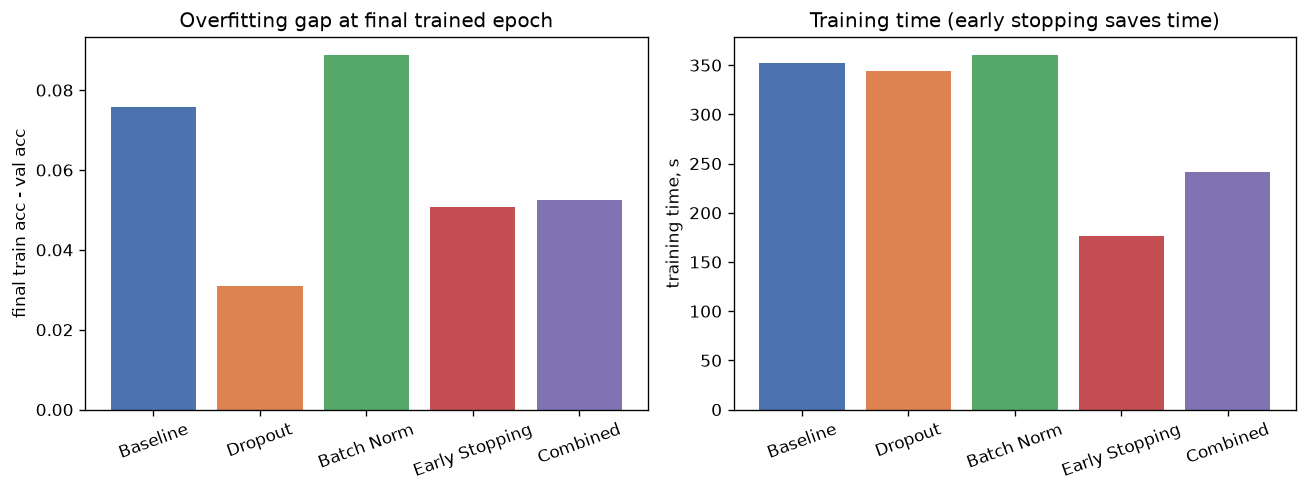
\includegraphics[width=0.95\textwidth]{figures/05_gap_and_time_summary.png}
    \caption{Left: final overfitting gap, all five. Right: training time, all five --
    early stopping's is by far the lowest.}
\end{figure}

\textbf{Recommendation.} \emph{Early Stopping is the most suitable single technique for
this problem}: it improved test accuracy over the baseline, cut the overfitting gap by
a third, and did it in half the training time, with no architectural change at all. If
a small amount of additional complexity is acceptable, the \emph{Combined}
configuration is the strongest overall choice -- it reaches within 0.13 points of Batch
Normalization's peak accuracy while keeping the overfitting gap contained (0.0525) and
finishing in two-thirds of Batch Normalization's training time. \emph{Batch
Normalization alone}, despite the best raw accuracy, is the hardest of the four to
recommend as a \emph{regularizer} on this evidence: it is solving a different problem
(optimization) than the one this task's overfitting baseline was built to expose.

\textbf{Advantages and limitations.}
\begin{itemize}
    \item \textbf{Dropout}: strong, direct variance reduction (smallest gap of all
    five); costs little extra compute per step; the downside here is it bought almost
    no test-accuracy improvement on its own, and typically needs more epochs to reach a
    given training loss since a fraction of units are silenced every step.
    \item \textbf{Batch Normalization}: the best accelerator of the four -- faster,
    higher-accuracy convergence -- but its reputation as a regularizer was not borne out
    on this task; use it for optimization stability and convergence speed, not as a
    substitute for an explicit regularizer against overfitting.
    \item \textbf{Early Stopping}: adds no parameters and no per-step compute, and was
    the only technique here that improved every axis simultaneously; its limitation is
    that it depends entirely on the validation split being representative, and it does
    not change what the model would have learned had training continued -- it simply
    stops at a good point along the same trajectory the baseline took.
    \item \textbf{Combined}: captures most of Batch Normalization's acceleration and
    most of Dropout's variance reduction at once, at the cost of being the most complex
    configuration to tune (an added dropout rate and patience value, rather than one or
    zero extra hyperparameters).
\end{itemize}

\textbf{Conclusion.} The thread running through this task is the same one that has run
through every task since Task 17: checking a claim against a measurement rather than
repeating it. ``Batch Normalization regularizes'' is a common enough claim that it would
have been easy to write it here without checking -- the measured gap says otherwise, on
this architecture and this dataset. The result that survives scrutiny is not a single
best technique in the abstract, but a specific, evidenced trade-off: Early Stopping for
the cheapest, most broadly positive single change; the combined configuration when the
extra accuracy is worth the extra tuning surface; and Batch Normalization treated as
what it measurably was here -- an optimizer aid, not a cure for overfitting.

\vspace{0.4cm}
\noindent The notebook and README are on GitHub: {\small\scalebox{0.72}[1]{\url{https://github.com/AbdullahAmir06/ai-internship-abdullahamir}}}

\end{document}
